\documentclass[a4paper, 16pt]{article}
\usepackage[utf8]{inputenc}
\usepackage[english, russian]{babel} 
\usepackage[left=20mm, top=20mm, right=20mm,
 bottom=20mm, head=1mm, foot=1mm]{geometry}
\usepackage{tikz} 
\usepackage{amsmath, amsfonts, amssymb}
\usepackage{graphicx}
\usepackage{fancybox, fancyhdr}
\usepackage{hyperref}
\usepackage{listings}
\usepackage{caption}
\usepackage{xcolor}
\pagestyle{fancy}
\fancyhf{}
\fancyhead[L]{Лабораторная работа №2}
\fancyhead[R]{Программирование промышленных контроллеров}
\fancyfoot[C]{\thepage}
\graphicspath{{images/}}
\usetikzlibrary{patterns}
\hypersetup{
    colorlinks=true,
    linkcolor=blue,
    filecolor=magenta,      
    urlcolor=cyan,
    pdftitle={contents setup},
    pdfpagemode=FullScreen,
}
\newcommand{\frc}[2]{\raisebox{2pt}{$#1$}\big/\raisebox{-3pt}{$#2$}}

\begin{document}
\begin{titlepage}

    \begin{center}
    \vfill
    
    Федеральное государственное автономное образовательное учреждение высшего образования\\
    «Национальный Исследовательский Университет ИТМО»\ \\
    
    \vfill
    {\large\bf ЛАБОРАТОРНАЯ РАБОТА №2\\
        ПО ПРЕДМЕТУ «ПРОГРАММИРОВАНИЕ ПРОМЫШЛЕННЫХ КОНТРОЛЛЕРОВ»}
    \vfill
        
    \begin{flushright}
        \begin{minipage}{.45\textwidth}
        {
            \hbox{Преподаватель: Крылова А. А.}
            \hbox{Выполнили:}
            \hbox{Румянцев А. А.}
            \hbox{Дьячихин Д. Н.}
            \hbox{}
            \hbox{Факультет: СУиР}
            \hbox{Потоки: ПРОГ. ПРОМ.ЛК 2.2 / 2.1}
        }
        \end{minipage}
    \end{flushright}
    
    \vfill
            
    Санкт-Петербург\\
    2024
    \end{center}
    \end{titlepage}
    \setlength{\parskip}{1.5mm}
    
    \tableofcontents

    \newpage
    \section{Установка}
    \noindent В данной лабораторной работе мы работали с стендом на основе ПЛК Schneider Electric Modicon M251


    \subsection{Схема установки}
    \begin{figure}[h!]
        \centering
        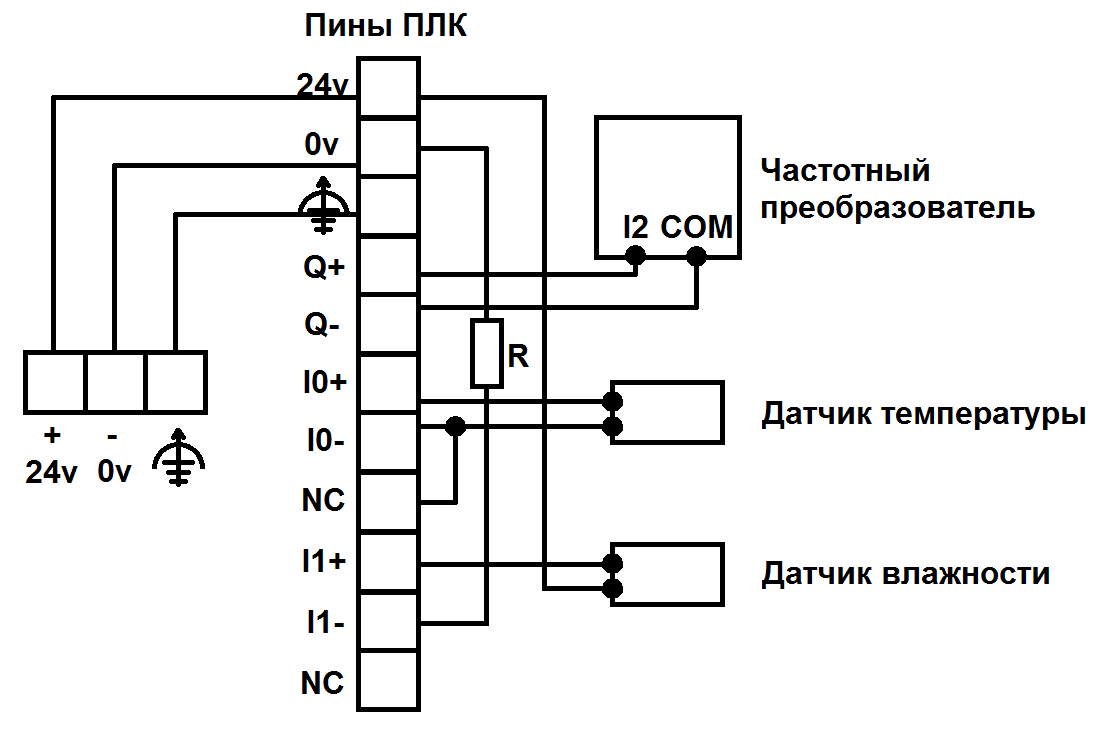
\includegraphics[scale=0.4]{схема_лаба2_плк.png}
        \captionsetup{skip=0pt}
        \caption{Схема стенда}
        \label{Рис:1}
    \end{figure}

    
    \subsection{Состав стенда}
    \begin{align*}
        & 1.\,\,\text{Контроллер Schneider Electric Modicon M251}\\
        & 2.\,\,\text{Блок аналогового ввода/вывода Schneider Electric TM3TM3}\\
        & 3.\,\,\text{Датчик температуры -- термосопротивление PT1000}\\
        & 4.\,\,\text{Датчик влажности TM1SH284 токовая петля 4--20мА}\\
        & 5.\,\,\text{Частотный преобразователь ALTIVAR ATV630 + асинхронный двигатель}
    \end{align*}


    \subsection{Пины}
    \begin{align*}
        & \circ\,\text{Термосопротивление \textbf{аналоговый вход I0} (диапазон [--2000, 6000], где 250 -- это 25.0 C)}\\
        & \circ\,\text{Датчик влажности \textbf{аналоговый вход I1} (диапазон [--150, 900], где 201 -- это 20.1 \% влажности)}\\
        & \circ\,\text{Чатотный преобразователь \textbf{аналоговый выход Q0} (диапазон [0, 24000], где 24000 -- это 10 В, 0 -- это 0 В)}
    \end{align*}


    \newpage
    \section{Задания}
    \subsection{Настройка проекта и его структура}
    \noindent Во всех заданиях сначала создается POU, потом в MAST с циклическим типом добавляется
    вызов файла соответствующего задания. Так выглядит MAST:
    \begin{figure}[h!]
        \centering
        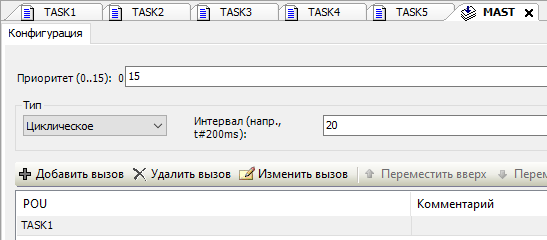
\includegraphics[scale=0.8]{mast.png}
        \captionsetup{skip=0pt}
        \caption{Вид файла MAST}
        \label{Рис:2}
    \end{figure}


    \noindent Структура лабораторной работы представлена на следующем рисунке:
    \begin{figure}[h!]
        \centering
        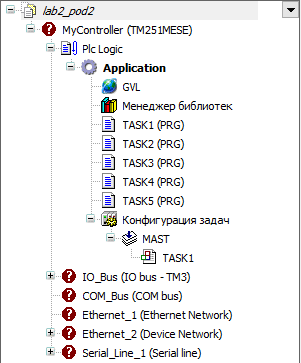
\includegraphics[scale=0.8]{structr.png}
        \captionsetup{skip=0pt}
        \caption{Структура проекта}
        \label{Рис:3}
    \end{figure}


    \noindent Перед выполнением лабораторной работы были настроены параметры датчика температуры, влажности и мотора. Переменная
    water\_{in} отвечает за входные данные с датчика влажности, temper\_{in} за входные данные с датчика температуры, motor ждет подачи значения.
    Минимальное значение попугаев двигателя 0, максимальное 24000. Минимальное значение температуры 230=23.0 градуса, максимальное 340=34.0


    \newpage
    \subsection{Задание 1}
    \noindent Вращать двигатель в течение 30 секунд на максимальной скорости, затем выключить.
    Для подсчета секунд нам понадобится переменная timer типа TP (пульс таймер), чтобы создать выходной
    сигнал тридцатисекундной длительности, и булевая переменная start, служащая входным сигналом для таймера
    \begin{figure}[h!]
        \centering
        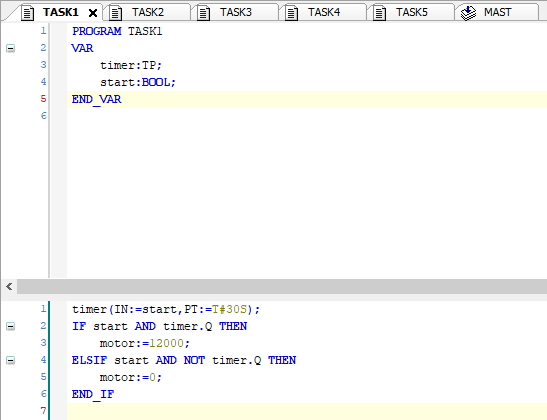
\includegraphics[scale=0.8]{t1.png}
        \captionsetup{skip=0pt}
        \caption{Код для задания 1}
        \label{Рис:4}
    \end{figure}


    \noindent Используем timer для вызова таймера, передаем перменную, к которой привязывается таймер, и
    задаем период таймера в 30 секунд. В условиях проверяется, что двигатель запущен и что таймер еще не досчитал
    до заданного времени. В результате выполнения кода двигатель проработал 30 секунд на 12000
    попугаях, после чего выключился


    \newpage
    \subsection{Задание 2}
    \noindent Вращать двигатель при влажности 80 \%, при снижении влажности до 50 \% выключить вращение двигателя. Для
    реализации нам не понадобятся дополнительные переменные, кроме той, что мы задали для отслеживания датчика влажности
    \begin{figure}[h!]
        \centering
        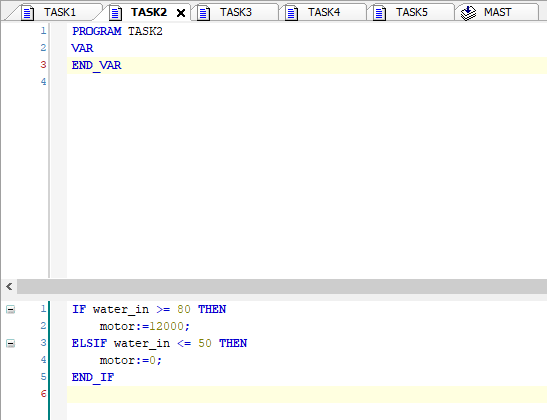
\includegraphics[scale=0.8]{t2.png}
        \captionsetup{skip=0pt}
        \caption{Код для задания 2}
        \label{Рис:5}
    \end{figure}


    \noindent Используем простые условия на проверку входящих данных с датчика влажности. Подаем на мотор
    попугаев или выключаем его при выполнении необходимых условий. В результате выполнения программы при превышении
    влажности в 80 \% двигатель начинал вращаться, пока датчик влажности не начинал показывать 50 \% и менее

    
    \newpage
    \subsection{Задание 3}
    \noindent Увеличивать скорость вращения двигателя пропорционально изменению значений с дачтика температуры.
    В данном задании нам нужно будет рассчитать коэффициент пропорциональности и привести полученное не целое число
    к целому для подачи попугаев на двигатель, поэтому переменная PROP имеет тип REAL
    \begin{figure}[h!]
        \centering
        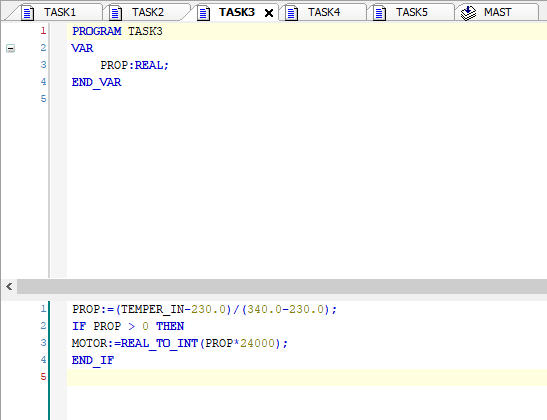
\includegraphics[scale=0.8]{t3.png}
        \captionsetup{skip=0pt}
        \caption{Код для задания 3}
        \label{Рис:6}
    \end{figure}


    \noindent Для расчета коэффициента пропорциональности мы воспользовались следующей формулой
    $$
    \text{PROP} = \frac{\text{TEMPER\_IN} - \text{TEMPER\_MIN}}{\text{TEMPER\_MAX} - \text{TEMPER\_MIN}}
    $$


    \noindent Так как температура с датчика может быть ниже минимальной, мы задали условие, что коэффициент
    должен быть строго больше нуля. На максимальное значение мы не написали проверку, но она имеет место быть, если
    двигатель должен работать в четко заданном диапазоне температур. Попугаев нужно подавать целым числом, поэтому используем
    REAL\_{TO}\_{INT}, причем сначала умножаем коэффициент на 24000, чтобы при маленьком коэффициенте он не округлялся до нуля и оборотов
    не было. В результате выполнения кода при повышении температуры
    двигатель повышал обороты, а при понижении температуры обороты снижались


    \newpage
    \subsection{Задание 4}
    \noindent Запустить асинхронный двигатель со скоростью 700 об/мин на 10 секунд, затем со
    скоростью 1400 об/мин на 20 секунд, затем выключить. В данном задании нам достаточно доработать
    нашу предыдущую наработку из задания 1, однако на мотор мы подаем попугаев, а нам сказали подавать обороты. Для начала
    переведем обороты в попугаи. На двигателе мы обнаружили следующую табличку:
    \begin{figure}[h!]
        \centering
        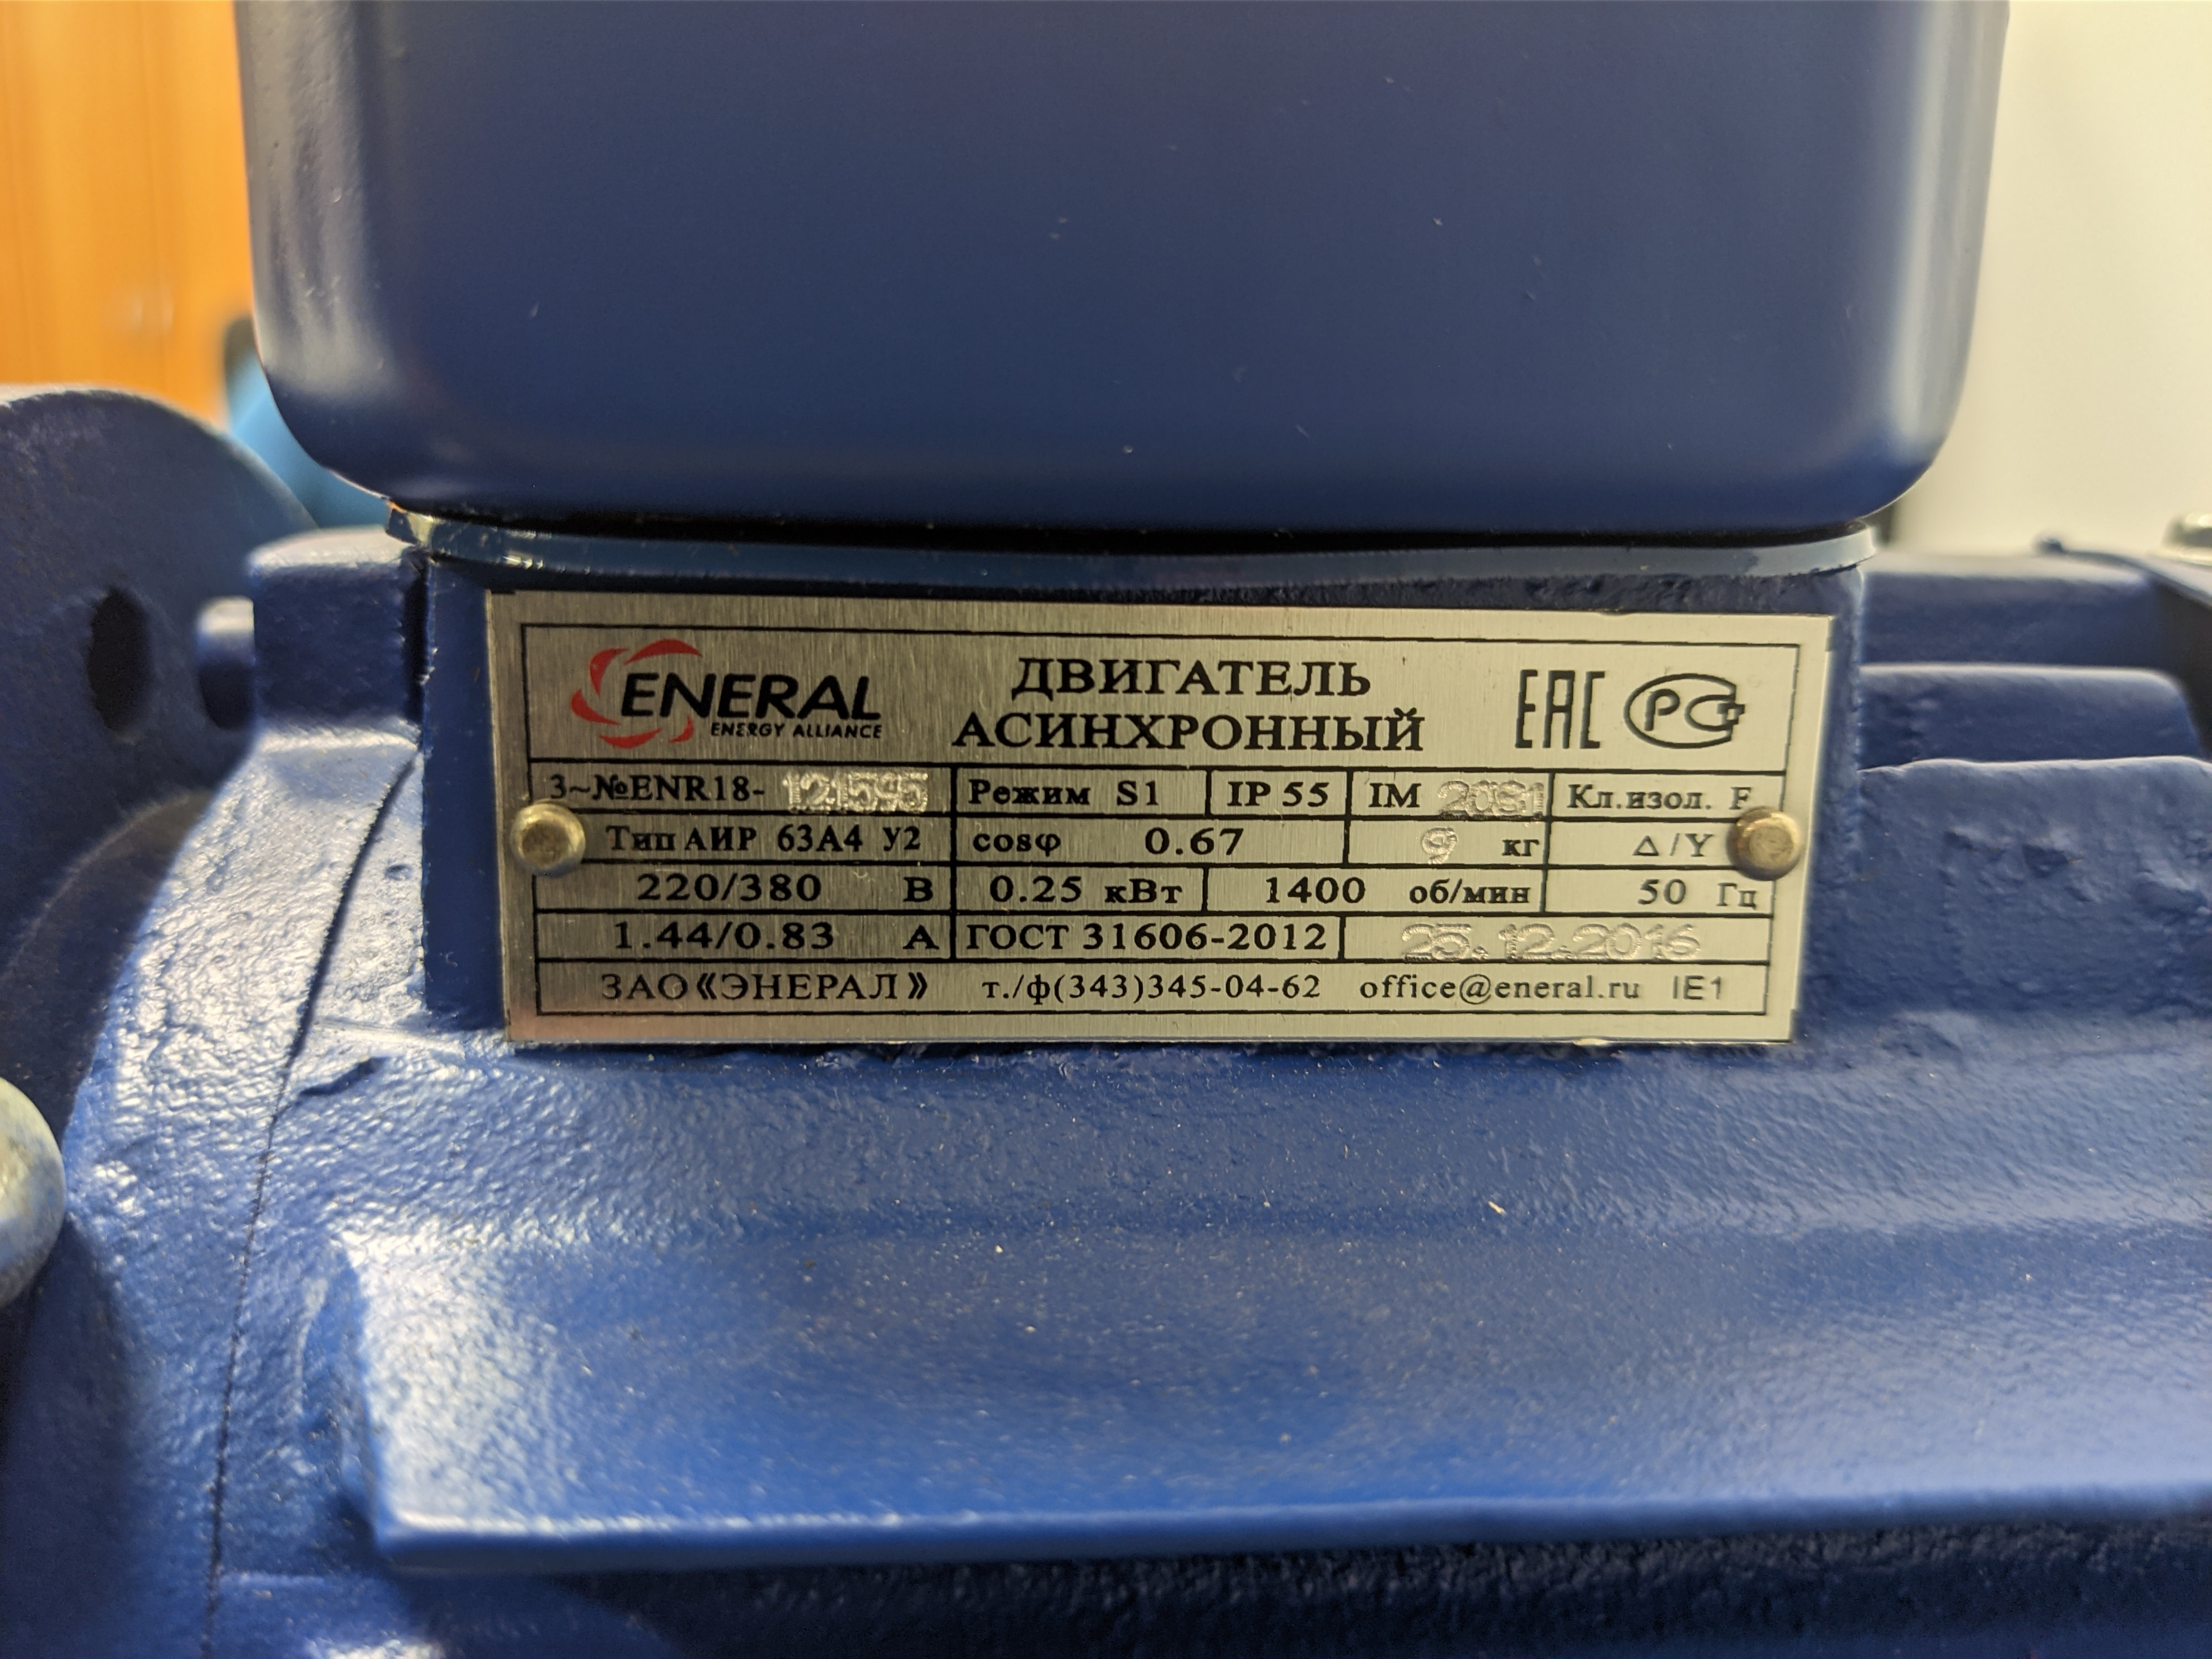
\includegraphics[scale=0.08]{photo.jpg}
        \captionsetup{skip=0pt}
        \caption{Табличка на асинхронном двигателе}
        \label{Рис:7}
    \end{figure}


    \noindent Видим, что 1400 об/мин это 50 Гц. Мы знаем, что 12000 попугаев это 100 Гц.
    2800 об/мин это 100 Гц, а значит $\frc{12000}{4}=3000$ попугаев соответствует $\frc{2800}{4}=700$ об/мин.
    Тогда 1400 об/мин это $3000\cdot2=6000$ попугаев. Теперь можем работать с кодом
    \begin{figure}[h!]
        \centering
        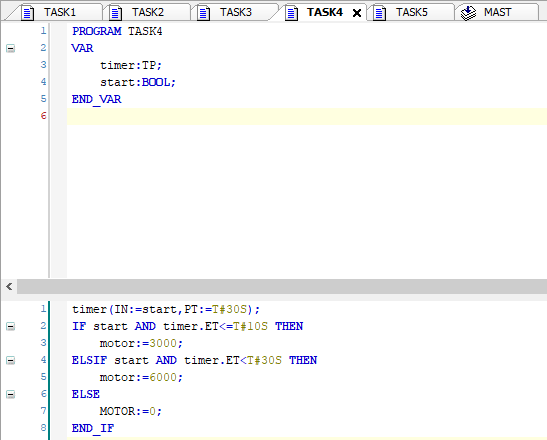
\includegraphics[scale=0.8]{t4.png}
        \captionsetup{skip=0pt}
        \caption{Код для задания 4}
        \label{Рис:8}
    \end{figure}


    \noindent В результате выполнения программы мотор 10 секунд вращася с низкой скоростью,
    потом 20 секунд с скоростью выше раза в два, затем выключился, в общей сумме провращавщись 30 секунд


    \newpage
    \subsection{Задание 5}
    \noindent Запустить асинхронный двигатель, менять скорость вращения пропорционально температуре. При
    достижении влажности в 80 \% снижать скорость вращения в 2 раза пропорционально температуре. Для выполнения
    задания нам достаточно скомбинировать код на таймер и код на пропорциональное повышение оборотов двигателя в зависимости
    от температуры и добавить проверку датчика влажности
    \begin{figure}[h!]
        \centering
        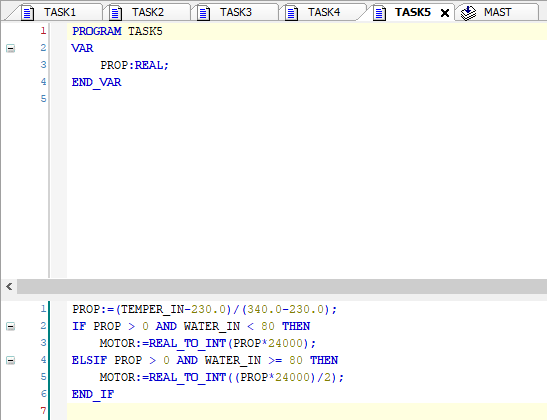
\includegraphics[scale=0.8]{t5.png}
        \captionsetup{skip=0pt}
        \caption{Код для задания 5}
        \label{Рис:9}
    \end{figure}


    \noindent В результате выполнения кода при показаниях датчика влажности менее 80 \% двигатель набирал обороты
    при повышении температуры, при понижении сбавлял обороты. По достижении влажности в 80 \% и более двигатель вращался
    в два раза медленнее с той же зависимостью, что и раньше


    \newpage
    \section{Вывод}
    \subsection{Лабораторная работа 2}
    \noindent В данной лабораторной работе мы познакомились с настоящим ПЛК, изучили работу установки -- за что отвечает
    каждый вход и каждый провод, поработали с асинхронным двигателем, отслеживали данные с датчиков, на основе которых взаимодействовали с установкой,
    закрепили умения настраивать файлы под необходимый сценарий и запускать программы с правильной последовательностью действий
\end{document}